% Per-agent model and multi-agent loop (fig:architecture), in the style of
% loop.tex. Adapted from Figure 3 of van Knippenberg et al. (2021), with the
% message-passing block of sec:method:model expanded.
% Build:  latexmk -pdf architecture.tex  -> architecture.pdf, copy to Images/.
\documentclass[border=2pt]{standalone}
\usepackage{lmodern}
\usepackage[T1]{fontenc}
\usepackage{amsmath,amssymb}
\usepackage{tikz}
\usetikzlibrary{positioning,fit,backgrounds,arrows.meta,calc,decorations.pathreplacing}

% Palette shared with base.py (C dict).
\definecolor{storeF}{HTML}{CFE3F7}
\definecolor{taskF}{HTML}{F6E7C1}
\definecolor{ctrlF}{HTML}{D7F0D8}
\definecolor{estF}{HTML}{F7D6D6}
\definecolor{delF}{HTML}{FFD9B3}
\definecolor{accent}{HTML}{2F6FAE}
\definecolor{ink}{HTML}{43505C}
\definecolor{muted}{HTML}{5A6673}

\tikzset{
  layer/.style={draw=ink, line width=0.8pt, rounded corners=3pt, align=center,
                fill=white, text width=5.2cm, minimum height=0.95cm,
                inner sep=3pt, font=\small},
  head/.style={draw=ink, line width=0.8pt, rounded corners=3pt, align=center,
               fill=ctrlF, text width=2.45cm, minimum height=1.05cm,
               inner sep=3pt, font=\small},
  agent/.style={draw=ink, line width=0.8pt, rounded corners=3pt, fill=ctrlF,
                minimum width=1.7cm, minimum height=0.8cm, font=\small},
  sys/.style={draw=ink, line width=0.8pt, rounded corners=3pt, align=center,
              minimum height=0.9cm, inner sep=4pt, font=\small},
  flow/.style={-{Stealth[length=2.4mm]}, line width=0.9pt, draw=ink},
  lbl/.style={font=\footnotesize, text=ink},
}

\begin{document}
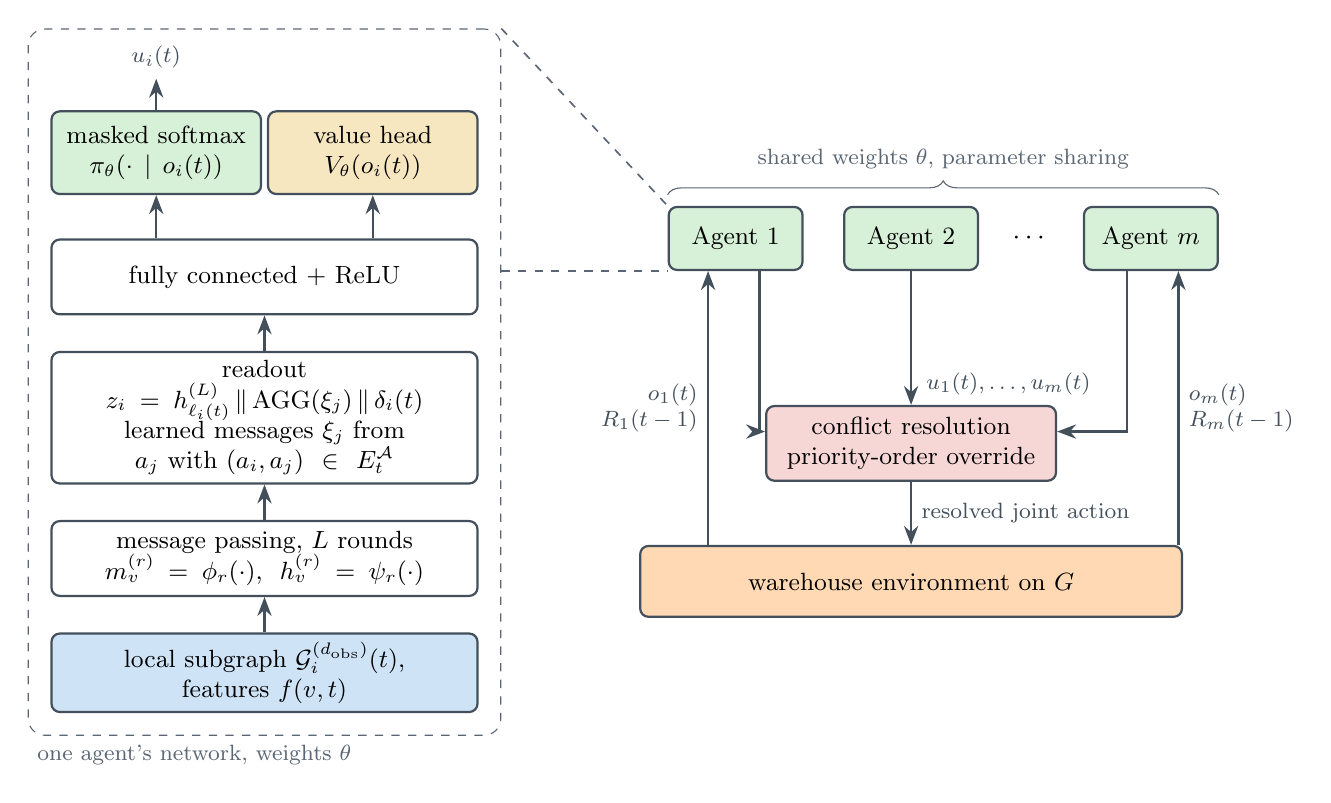
\begin{tikzpicture}
  % ---------------------------------------------------------- the network
  \node[layer, fill=storeF] (in) {local subgraph
    $\mathcal{G}_i^{(d_{\mathrm{obs}})}(t)$, features $f(v,t)$};
  \node[layer, above=0.45cm of in] (mp) {message passing, $L$ rounds\\
    $m_v^{(r)} = \phi_r(\cdot)$, \ $h_v^{(r)} = \psi_r(\cdot)$};
  \node[layer, above=0.45cm of mp] (ro) {readout\\
    $z_i = h^{(L)}_{\ell_i(t)} \,\Vert\, \mathrm{AGG}(\xi_j) \,\Vert\, \delta_i(t)$\\
    learned messages $\xi_j$ from $a_j$ with $(a_i,a_j)\in E^{\mathcal{A}}_t$};
  \node[layer, above=0.45cm of ro] (fc) {fully connected + ReLU};
  \node[head, above=0.55cm of fc.north west, anchor=south west] (pi)
    {masked softmax\\ $\pi_\theta(\cdot \mid o_i(t))$};
  \node[head, fill=taskF, above=0.55cm of fc.north east, anchor=south east] (V)
    {value head\\ $V_\theta(o_i(t))$};

  \draw[flow] (in) -- (mp);
  \draw[flow] (mp) -- (ro);
  \draw[flow] (ro) -- (fc);
  \draw[flow] (fc.north -| pi) -- (pi);
  \draw[flow] (fc.north -| V) -- (V);
  \draw[flow] (pi.north) -- ++(0,0.4) node[above, lbl] {$u_i(t)$};

  \coordinate (nettop) at ($(pi.north)+(0,0.75)$);
  \begin{scope}[on background layer]
    \node[draw=muted, dashed, rounded corners=6pt, inner sep=8pt,
          fit=(in)(pi)(V)(nettop)] (net) {};
  \end{scope}
  \node[font=\footnotesize, text=muted, anchor=north west]
    at (net.south west) {one agent's network, weights $\theta$};

  % ---------------------------------------------------------- the loop
  \node[agent, right=2.4cm of fc.north east, anchor=west] (a1) {Agent $1$};
  \node[agent, right=0.5cm of a1] (a2) {Agent $2$};
  \node[right=0.3cm of a2] (dots) {$\cdots$};
  \node[agent, right=0.3cm of dots] (am) {Agent $m$};

  \draw[decorate, decoration={brace, amplitude=5pt, raise=4pt}, draw=muted]
    (a1.north west) -- (am.north east)
    node[midway, above=10pt, font=\footnotesize, text=muted]
    {shared weights $\theta$, parameter sharing};

  \node[sys, fill=estF, text width=3.4cm, below=1.7cm of a2] (cr)
    {conflict resolution\\ priority-order override};
  \node[sys, fill=delF, text width=6.6cm, below=0.8cm of cr] (env)
    {warehouse environment on $G$};

  % observations and rewards up to each agent
  \draw[flow] (env.north -| a1) ++(-0.35,0) -- ($(a1.south)+(-0.35,0)$)
    node[pos=0.5, left, lbl, align=right] {$o_1(t)$\\ $R_1(t-1)$};
  \draw[flow] (env.north -| am) ++(0.35,0) -- ($(am.south)+(0.35,0)$)
    node[pos=0.5, right, lbl, align=left] {$o_m(t)$\\ $R_m(t-1)$};

  % proposed actions down into resolution, resolved action into env
  \draw[flow] ($(a1.south)+(0.3,0)$) |- ($(cr.west)+(0,0.15)$);
  \draw[flow] (a2.south) -- (cr.north);
  \draw[flow] ($(am.south)+(-0.3,0)$) |- ($(cr.east)+(0,0.15)$);
  \node[lbl, above right=0pt and 2pt of cr.north] {$u_1(t),\dots,u_m(t)$};
  \draw[flow] (cr) -- node[right, lbl] {resolved joint action} (env);

  % zoom lines from the network to agent 1
  \draw[muted, dashed, line width=0.6pt] (net.north east) -- (a1.north west);
  \draw[muted, dashed, line width=0.6pt] (a1.south west -| net.east) -- (a1.south west);
\end{tikzpicture}
\end{document}
